\chapter{Methodology}
In this section a methodology is given how to describe the deployment of deep learning models on either edge devices or on a cloud-backend.
\section{Problem Space}
The inference performance of a deep learning model is mainly affected by two major parts, the model itels and the hardware environment where it gets deployed. A third factor is the serving framework.
\begin{itemize}
    \item Warum die Frage Edge oder Cloud
\end{itemize}
\section{Deep Learning}
Deep learning models describe neural network with many layers and hidden units, the most popular being convolutional neural networks and recurrent neural networks right now. This increased amount of layers leads to complex mathematical calculations.


\begin{figure}[H]
\centering
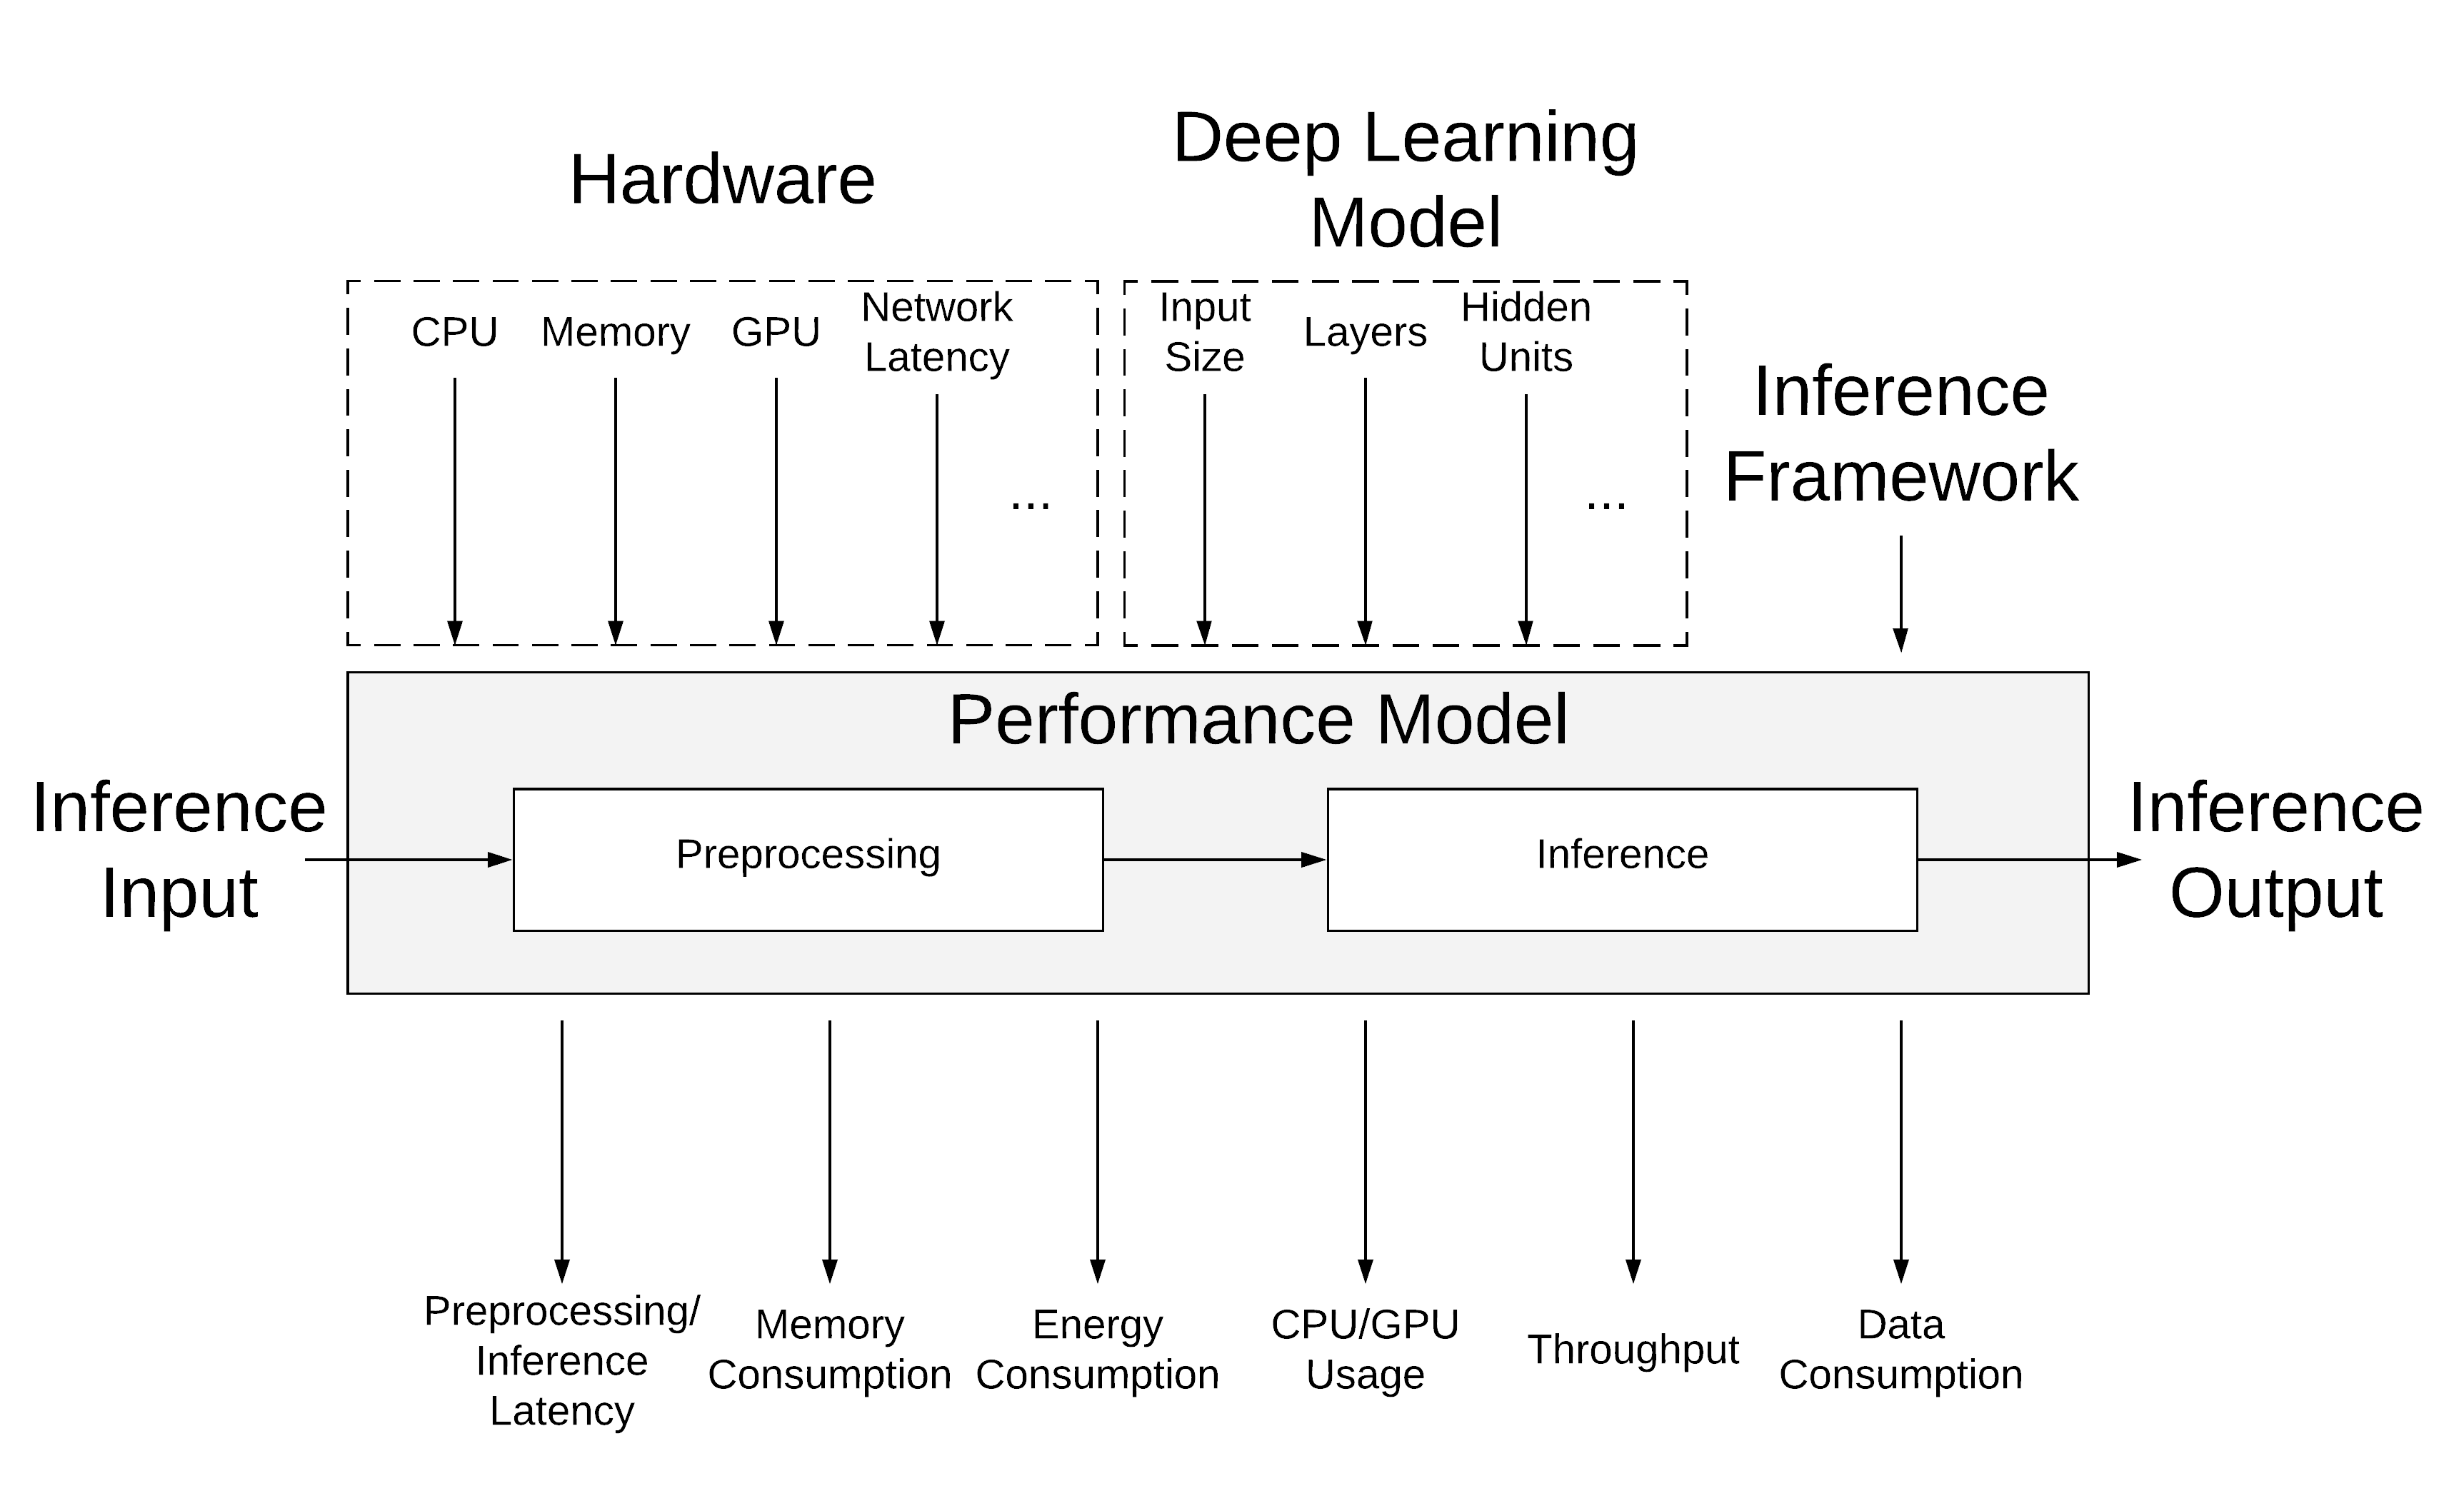
\includegraphics[width=0.9\textwidth]{./Bilder/trade_offs.png}
\caption{placeholder}
\label{fig:trade_offs}
\end{figure}
\begin{figure}[H]
\centering
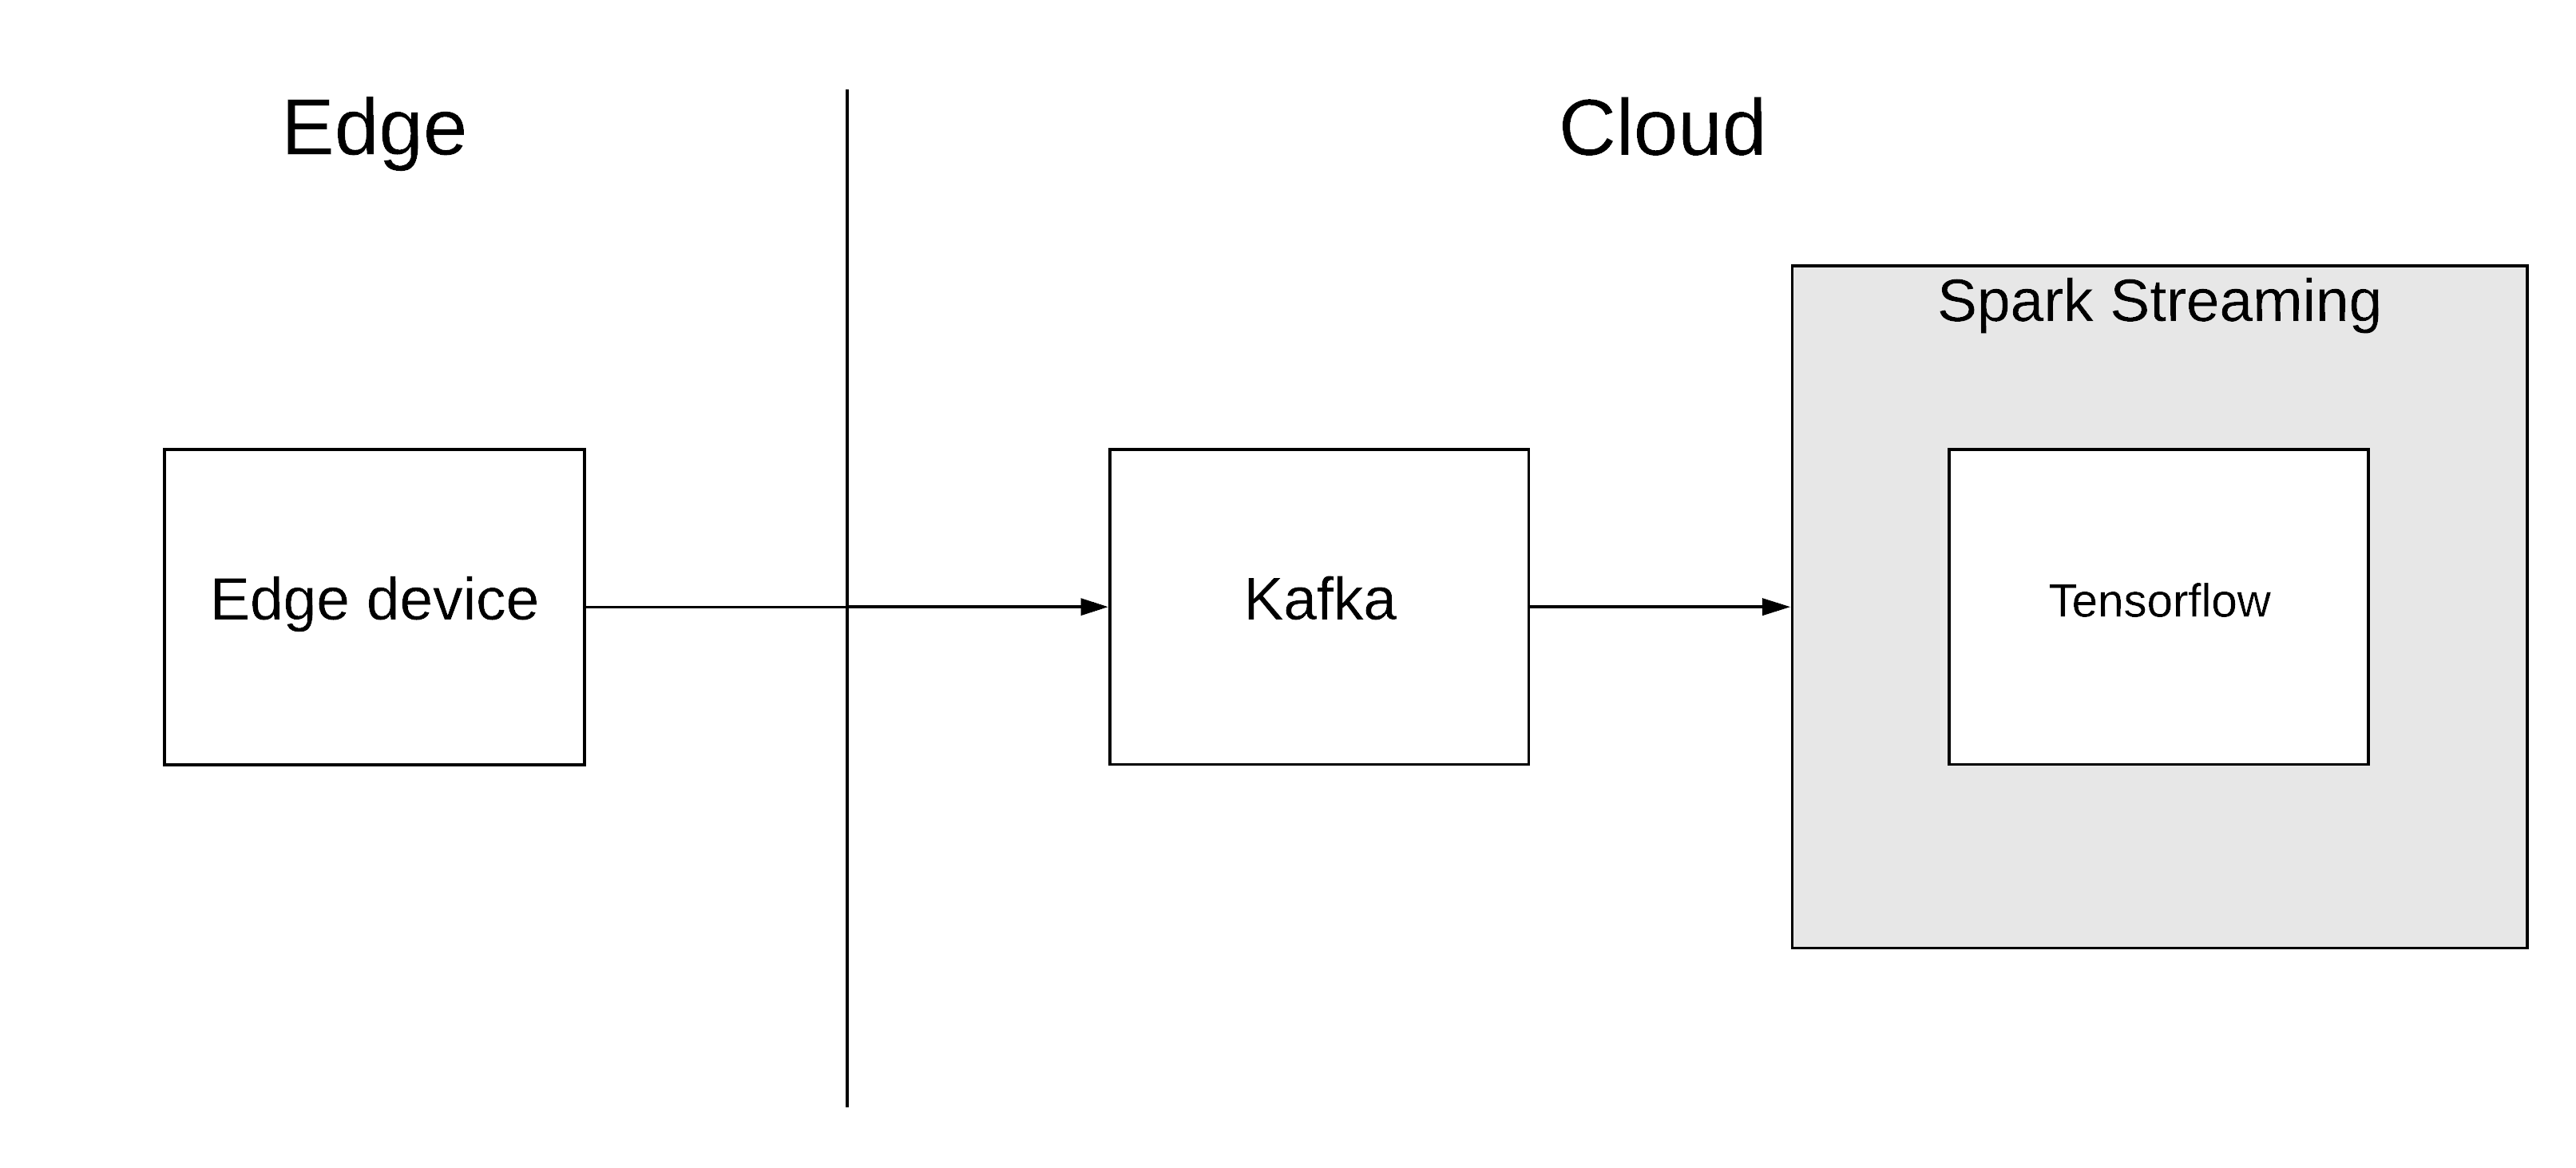
\includegraphics[width=0.9\textwidth]{./Bilder/spark_stream.png}
\caption{placeholder}
\label{fig:trade}
\end{figure}
\begin{itemize}
    \item parameter von Modellen
    \item Was für Einfluss haben diese Parameter?
\end{itemize}
\section{Deployment}
Model deployment describes the process of deploying a trained machine learning model to a production environment.
\subsection{Edge Deployment}+
\begin{itemize}
    \item Was ist Edge (Beispiele)
    \item Was macht Edge aus?
\end{itemize}
\subsection{Cloud Deployment}
\begin{itemize}
    \item Was ist cloud?
    \item Was macht cloud aus
\end{itemize}
\section{Deployment Trade-offs}
\begin{itemize}
    \item Unterschiede aus verschiedenen deployment optionen
\end{itemize}
Metriken:
\begin{itemize}
    \item Welche Metriken (inference time....)
    \item Wie werden die Metriken gemessen?
    \item Wo werden Metriken gemessen?
\end{itemize}

\endinput 